\documentclass[conference]{IEEEtran}
\IEEEoverridecommandlockouts
% The preceding line is only needed to identify funding in the first footnote. If that is unneeded, please comment it out.
\usepackage{cite}
\usepackage{amsmath,amssymb,amsfonts}
\usepackage{algorithmic}
\usepackage{graphicx}
\usepackage{textcomp}
\usepackage{xcolor}
\def\BibTeX{{\rm B\kern-.05em{\sc i\kern-.025em b}\kern-.08em
    T\kern-.1667em\lower.7ex\hbox{E}\kern-.125emX}}
\begin{document}

\title{Literature Review: Scenario Description Languages
}

\maketitle

\begin{abstract}
Recently, the rapid development of autonomous vehicles (AVs) has inspired many researchers in this field and made it more efficient and safe. To gain more reliability and safety during autonomous driving (AD), AVs need many sensors and equipment to be fully aware of the environment. Although the existing tools to verify and test AVs as a whole can simulate different scenarios well, they do not provide an integrating platform to consider cybersecurity issues from the perspective of each sensor during simulation. Therefore, this work will sort out the challenges and problems Scenario Description Languages (SDL) face and propose a feasible future for how to improve these languages.
\end{abstract}

\begin{IEEEkeywords}
Scenario Description Languages, LiDAR, cybersecurity
\end{IEEEkeywords}

\section{Introduction}
Scenario Description Languages (SDL) have become popular due to the increasing need for more reliable and safer autonomous driving (AD). Even though the existing SDL tools could generate scenarios and test the margin case of autonomous vehicles (AVs) as a whole, they have not considered the cybersecurity perspective for AVs\cite{b1,b6}. For example, as one of the popular sensors, LiDAR (Light Detection And Ranging) is in danger of a spoofing attack. Still, there is no systematic way to describe this as a scenario in the existing SDL tools. \cite{b2} Besides, some research also points out that an unnoticeable attack on cameras, as one of the popular equipment, in real life could pose a risk for AVs by misclassification\cite{b5}. Therefore, how to abstract these cybersecurity attacks into scenarios systematically and using them in SDL will be the focus in Section\ref{sec: Challenges and Solutions}.
\section{Previous Work}
\label{sec: PW}
When it comes to the verification and testing of AVs, how to precisely describe the situations is of utmost importance. In the following context, \textbf{scenario} will be the word to replace situations above to follow the terms in this field.
\begin{figure}[htbp]
\centerline{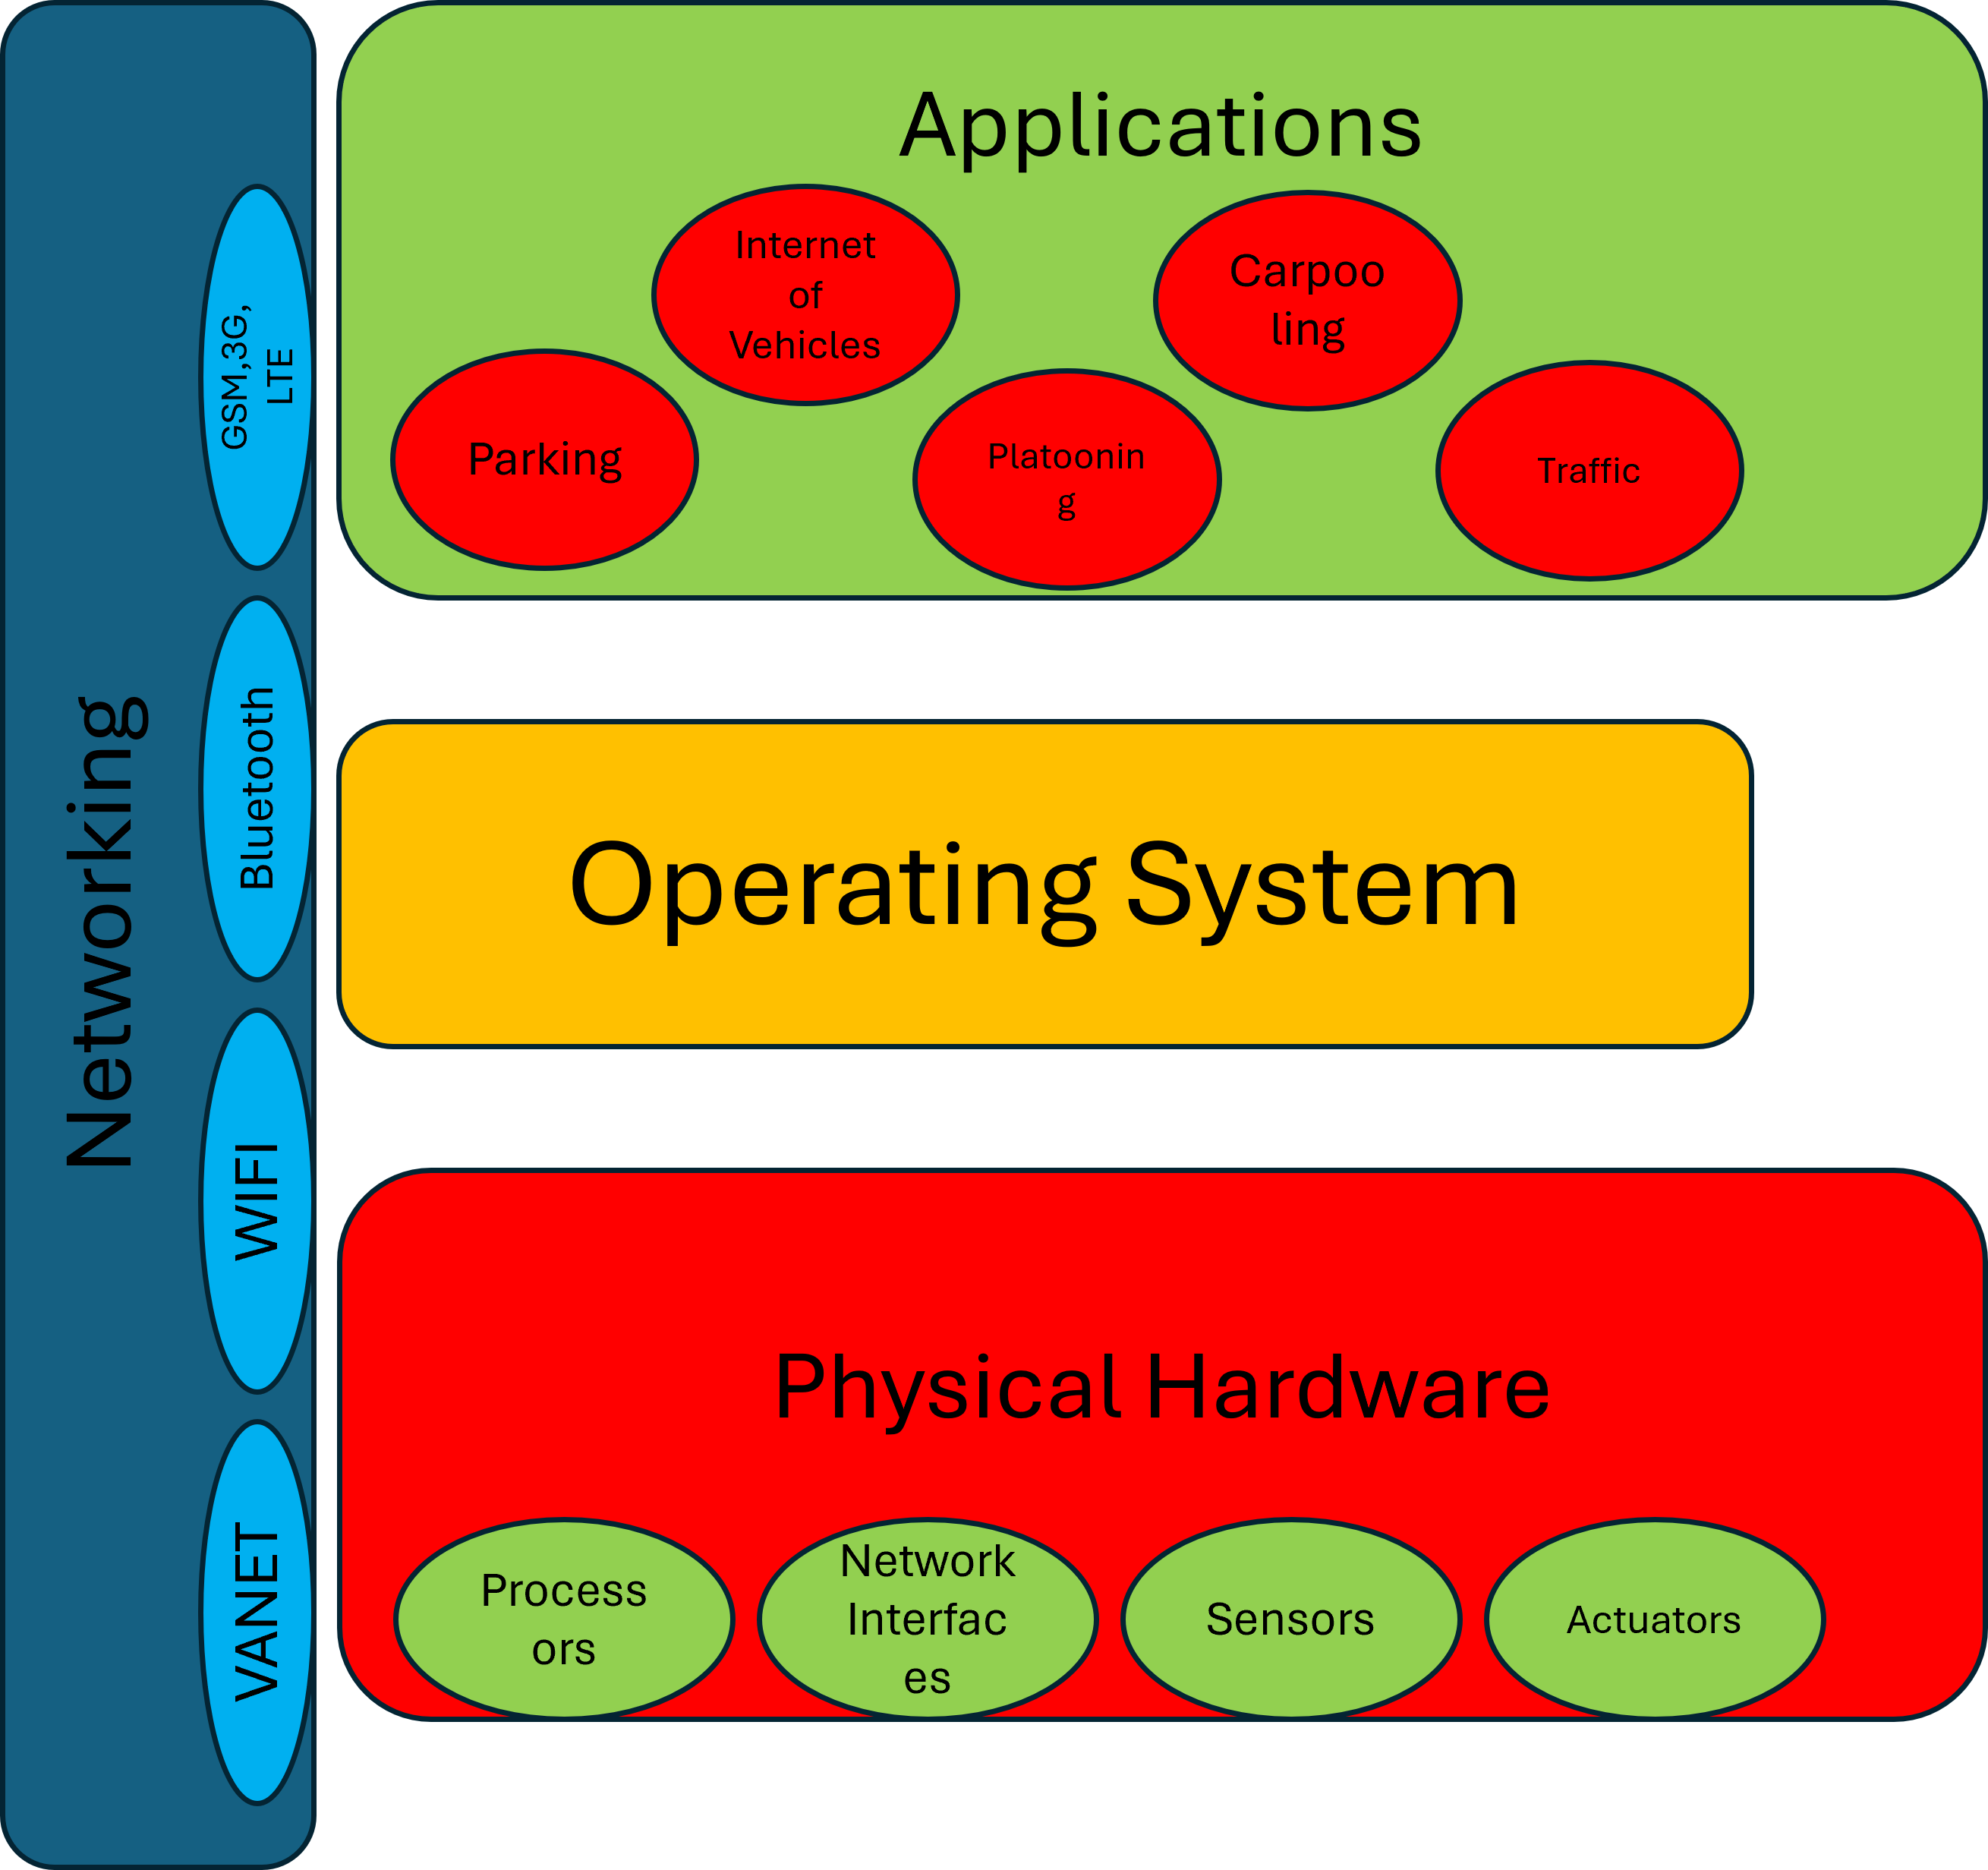
\includegraphics[width=80mm,scale=0.5]{./pic/pic1_layers.png}}
\caption{the extended layers for AVs \cite{b7}. SDL tools mostly focus on the scenarios in the Applications layer, like parking and traffic.}
\label{fig1}
\end{figure}
As Fig.\ref{fig1} has shown, the elements of AVs could be separated into 4 layers: \textbf{Networking, Applications, Operating System and Physical Hardware}. 
So far, the tools of SDL have expressed the great capability of simulating the scenarios based on the vehicles for the cases, such as controlling the values of positions, angles, and actions from different cars. Nevertheless, the majority of controllable factors from SDL tools lie in the Application Layer, leaving other layers unverified. This lack of integrity could underestimate the potential attacks in real life and put  AVs in danger, especially for the Physical Hardware Layer, where the attack could happen while driving without any detection from software systems and notice from drivers. Therefore, the research and study of the attacks against these Physical Hardware are invaluable for future improvements of SDL tools. Here, LiDAR and cameras as the two most popular equipment on Avs will be discussed. Finally, the case studies into generating Scenarios and modeling the perception of LiDAR make it possible to propose some feasible solutions to tackle challenges in SDL tools in the future.
\subsection{SDL tools}
SDL tools mainly utilize the probabilistic programming language to evaluate cyber-physical systems and solve the overhead of Machine Learning (ML) based systems due to a huge amount of collection time for training data. Among all tools, \textbf{SCENIC} is one of the popular tools  \cite{b6}, so the following introduction will be based on it.
Usually, these SDL tools can describe vehicles from 2 basic perspectives:  \textbf{properties} and  \textbf{actions}. Take SCENIC as an example, it can control the speed, heading direction with degrees, and visibility of other vehicles as properties while making actions, like following another car, at the same time. These tools could then form different requirements from these 2 perspectives. For example, it is quite easy to construct a condition that the car will follow other cars only if other cars are close to it within 15 m. Specifically, these requirements should also be classified into soft and hard ones. If a requirement has to be met in each moment, which is referred to as a \textbf{scene}, it is a hard requirement. Otherwise, it is a soft one. In SCENIC, these hard requirements could then be used to speed up the simulation by filtering out scenes violating them, which is known as scenario improvisation.
\begin{figure}[htbp]
\centerline{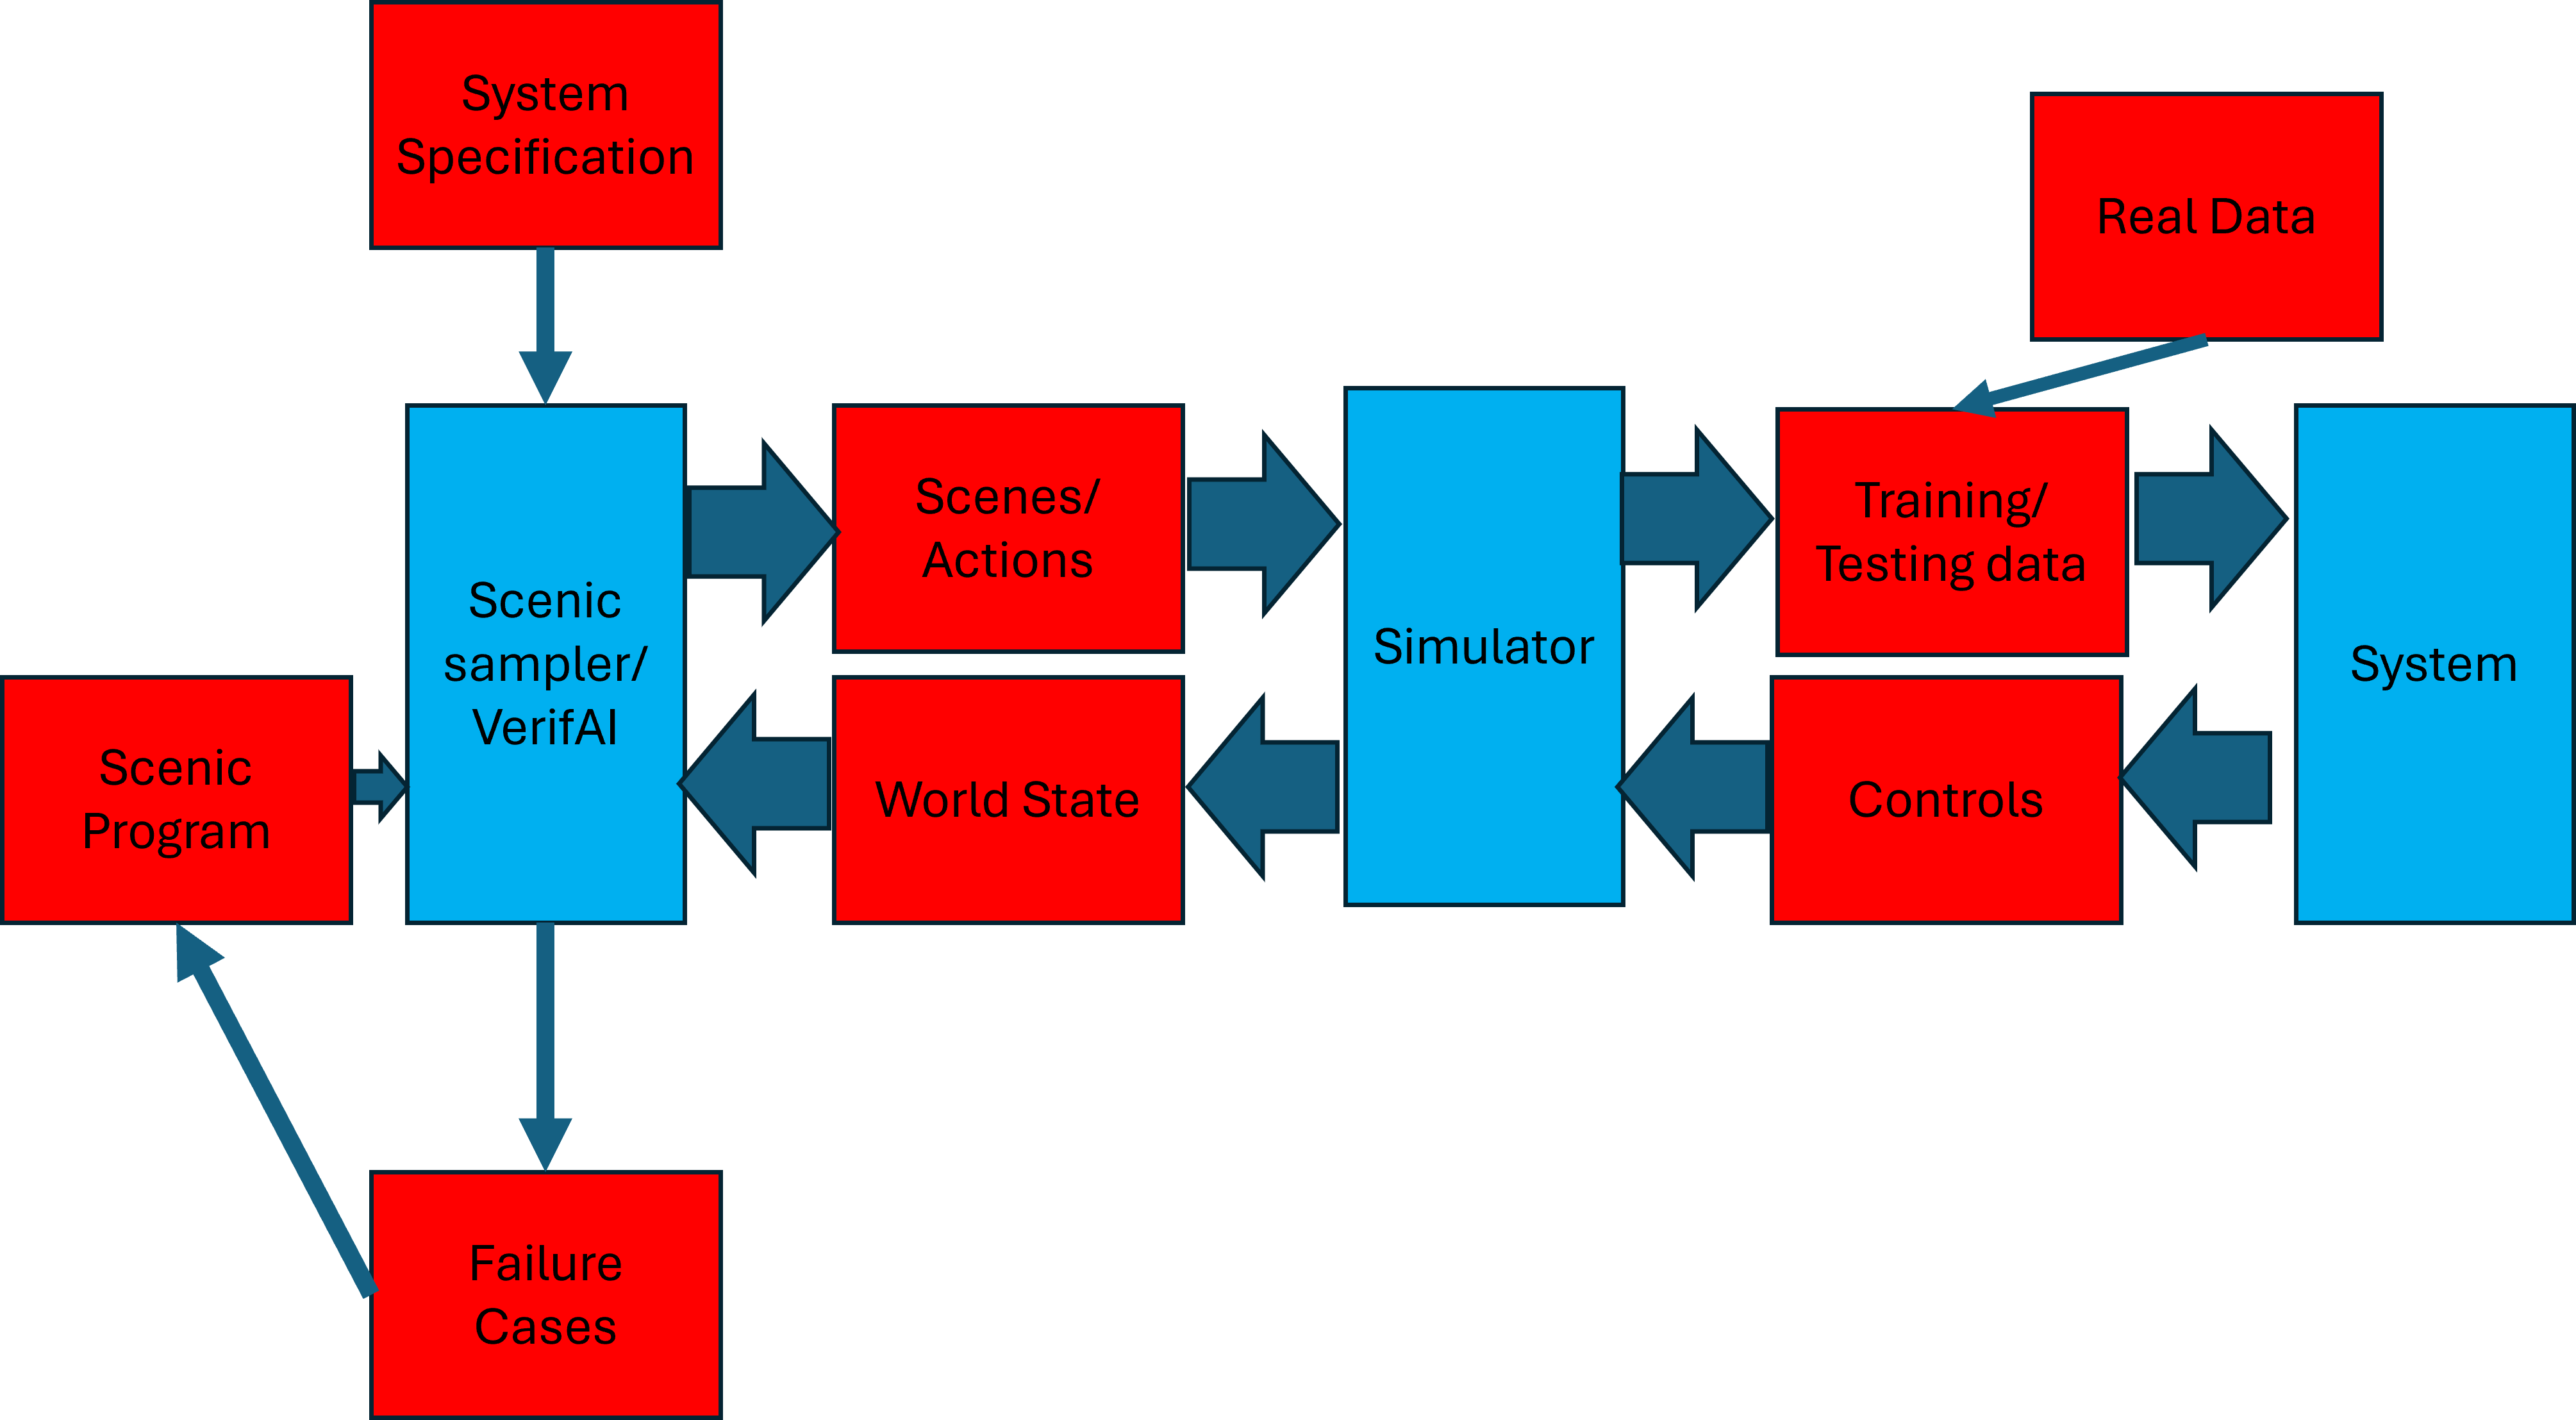
\includegraphics[width=90mm]{./pic/pic2_scenicflow.png}}
\caption{the flow of usage with SDL tools for training ML-based cyber-physical systems. As the flow indicates, it is easy to get the margin cases and faliure cases by the feedback of the flow.}
\label{fig2}
\end{figure}

The flow in Fig.\ref{fig2} is an example of the usage of SDL tools, and it shows that these tools are such good options for training an ML-based model and finding out the edge cases that may cause collisions or fail the requirements quite easy.
\subsection{Physical Hardware Attack}
The attacks on the Physical Hardware could be identified as black-box or white-box attacks. Usually, black-box attacks could happen more easily than white-box ones since they do not require information about the vehicles of victims. Consideration of the security against these attacks should be the priority in most cases, but it is always hard to come up with a well-designed technique without a correct model from real life: for example, LiDAR, as a sensor that uses the reflection of a laser to provide detailed 3D information for the surrounding environment, is already equipped with simultaneous laser firing, timing randomization or pulse fingering nowadays to prevent the synchronization property of white-box attacks\cite{b8,b9,b10}. However, some experiments have indicated that all these new generations of LiDAR cannot defend itself from the asynchronous black-box attacks \cite{b2}. In addition, in these experiments, synchronous and asynchronous attacks have been carried out by the proper experiment setup with an additional amplifier, and in the end, the previous research and models of LiDAR have been proved misleading from the real world because of the insufficient consideration of errors. Another example comes from cameras. Even though an early study has shown that attackers could even put some malicious attacks under graffiti or posters to trick the classifier of cameras in theory, the directions to tackle this issue were still unclear at that time without real-life experiments \cite{b5}. From the examples above, if any of the attacks successfully happen in busy traffic, it could result in a serious accident easily. Therefore, most of the design for AVs should be equipped with more than one sensors and aids. With the help of a classifier of a camera, the additional check of correctness and functionality of detecting an attack could become true on the point cloud from LiDAR.  Given that modern AVs have considered the consistency between different sensors, there have been studies on the attacks on multiple devices. One of these remarkable attacks is Frustum Attack \cite{b1}. This attack fully utilize the knowledge from both cameras and LiDAR as there exists an overlapping area called a frustum, where both equipment will detect the nearby area with high uncertainty. In other words, if we surround the shadow area with a bounding box from the view in cameras, we could find out that inside this bounding box, the attacks to manipulate the cloud points of LiDAR have a very high probability of succeeding. To summarize, all these attacks target the weaknesses and characteristics of each device. For LiDAR, the lack of checking the sender of a received signal and the usage of the reflection could let prevention of attacks be quite hard. As for cameras, the clearness of every picture and the robustness of a classifier are both hard to maintain and improve. Thus, the precautions for these attacks while happening are necessary, and to achieve this, the systematic ways to model attacks and get failed cases should not be overlooked.
\subsection{Generation of Scenarios and a LiDAR Model}
For the purpose of constructing scenarios of attacks systematically, there are several organized ways to treat a scenario. Among them, the OpenScenario standard has been widely used to generate AD test scenarios \cite{b11}. It separates a scenario into 3 main parts: Road, Environment, and Traffic Participants. The first two elements are highly related to the property perspective in SDL tools, and as for actions, the last one includes the behavioral descriptions for each participant. Therefore, as long as the configuration files can be obtained and analyzed, generating multiple cases with changing of uncontrollable factors is possible. 
\begin{table}[htbp]
\caption{the five types of AD simulation tests in industry \cite{b4}.}
\begin{center}
\begin{tabular}{|l|p{3.4cm}|p{3.4cm}|}
\hline
\textbf{num} & \textbf{\textit{name}}& \textbf{\textit{pourpose}} \\
\hline
\textbf{1} & \textbf{\textit{Model-in-the-loop}}& \textbf{\textit{Integration tests for model-level tasks.}} \\
\hline
\textbf{2} & \textbf{\textit{Software-in-the-loop}}& \textbf{\textit{Verify that the generated code and the model are functionally consistent.}} \\
\hline
\textbf{3} & \textbf{\textit{Hardware-in-the-loop}}& \textbf{\textit{Validate the controller.}} \\
\hline
\textbf{4} & \textbf{\textit{Driver-in-the-loop}}& \textbf{\textit{Verify the system.}} \\
\hline
\textbf{5} & \textbf{\textit{Vehicle-in-the-loop}}& \textbf{\textit{Verify the function of the test system, the simulation test of each scenario, the matching and integration test with the relevant electronic control system of the vehicle.}} \\
\hline
\end{tabular}
\label{tab1}
\end{center}
\end{table}
In terms of industry, the 5 types of AD simulation tests are listed in Table \ref{tab1}, and quite often, Model-in-the-loop is the type SDL-related tools are used for. For example, generating test cases in this type of AD simulation could be performed with the OpenScenario standard as well as traversing algorithms to get behavioral systems \cite{b4}. However, the capability of describing a scenario also counts on a reliable model to simulate or even predict the following scenes with the given conditions. A generative model that predicts the next observation in an environment given past observations and the current action is called a world model in this sense.  While the simulation models on cameras based on the process of real cameras gained great success a long time ago \cite{b12}, the precise world model on LiDAR from the modification of the diffusion model has just been launched recently, called Copilot4D \cite{b3}. Let $\mathrm {x^{(t)}}$ be tokenized observation at time $\mathrm{t}$, and $\mathrm {a^{(t)}}$ be actions at time $\mathrm{t}$. With $\mathrm{\tau=(x^{(1)},a^{(1)}.....x^{(t)},a^{(t)})}$ as the history until now and $\mathrm{c^{(t-1)}=(x^{(1)},a^{(1)}.....x^{(t-1)},a^{(t-1)})}$ as history agents, a diffusion model with function $\mathrm{P}$ will learn to predict the $\mathrm{x_{0}^{(t)}}$ until $\mathrm{x_{k}^{(t)}}$:
\begin{equation}
\begin{aligned}
E_{q(\tau)}[\Sigma_{t=1}P(x^{(t)}|c^{(t-1)})]>=\\
E_{q(\tau)}[\Sigma_{t=1}\Sigma_{k=1}E_{q(x_{k}^{(t)},x_{0}^{(t)})}[P(x_{0}^{(t)}| x_{k}^{(t)},c^{(t-1)})]+C]
\end{aligned}
\label{eq1}
\end{equation}
The left-hand side of \eqref{eq1} means the future prediction while the right-hand side is a discrete diffusion on each observation. The whole equation, similar to Masked Generative Image Transforme \cite{b13}, could then be used as a Generative Pre-trained Transformers (GPT)-like formulation of autoregressive modeling. The main idea of this world model is around \eqref{eq1} and builds up an unsupervised generative model. The better performance of prediction comes from the training for discrete time frames with the mixing up of temporal data.
\section{Challenges and Solutions}
\label{sec: Challenges and Solutions}
The challenges of SDL under the following discussion can then be summarized according to Section\ref{sec: PW}:
\begin{itemize}
\item limited objective layers in the scenarios  $\mathrm{-}$ The target of the SDL tools is application layer mostly, so there is no existing functions to describe a scenario within the Physical Hardware layer.
\item lack of systematic way to describe the attack scenarios $\mathrm{-}$ SDL tools are limited to a much high level to perform simulation, so there is no mechanism and grammar for lower levels and other layers.
\end{itemize}
\begin{figure}[htbp]
\centerline{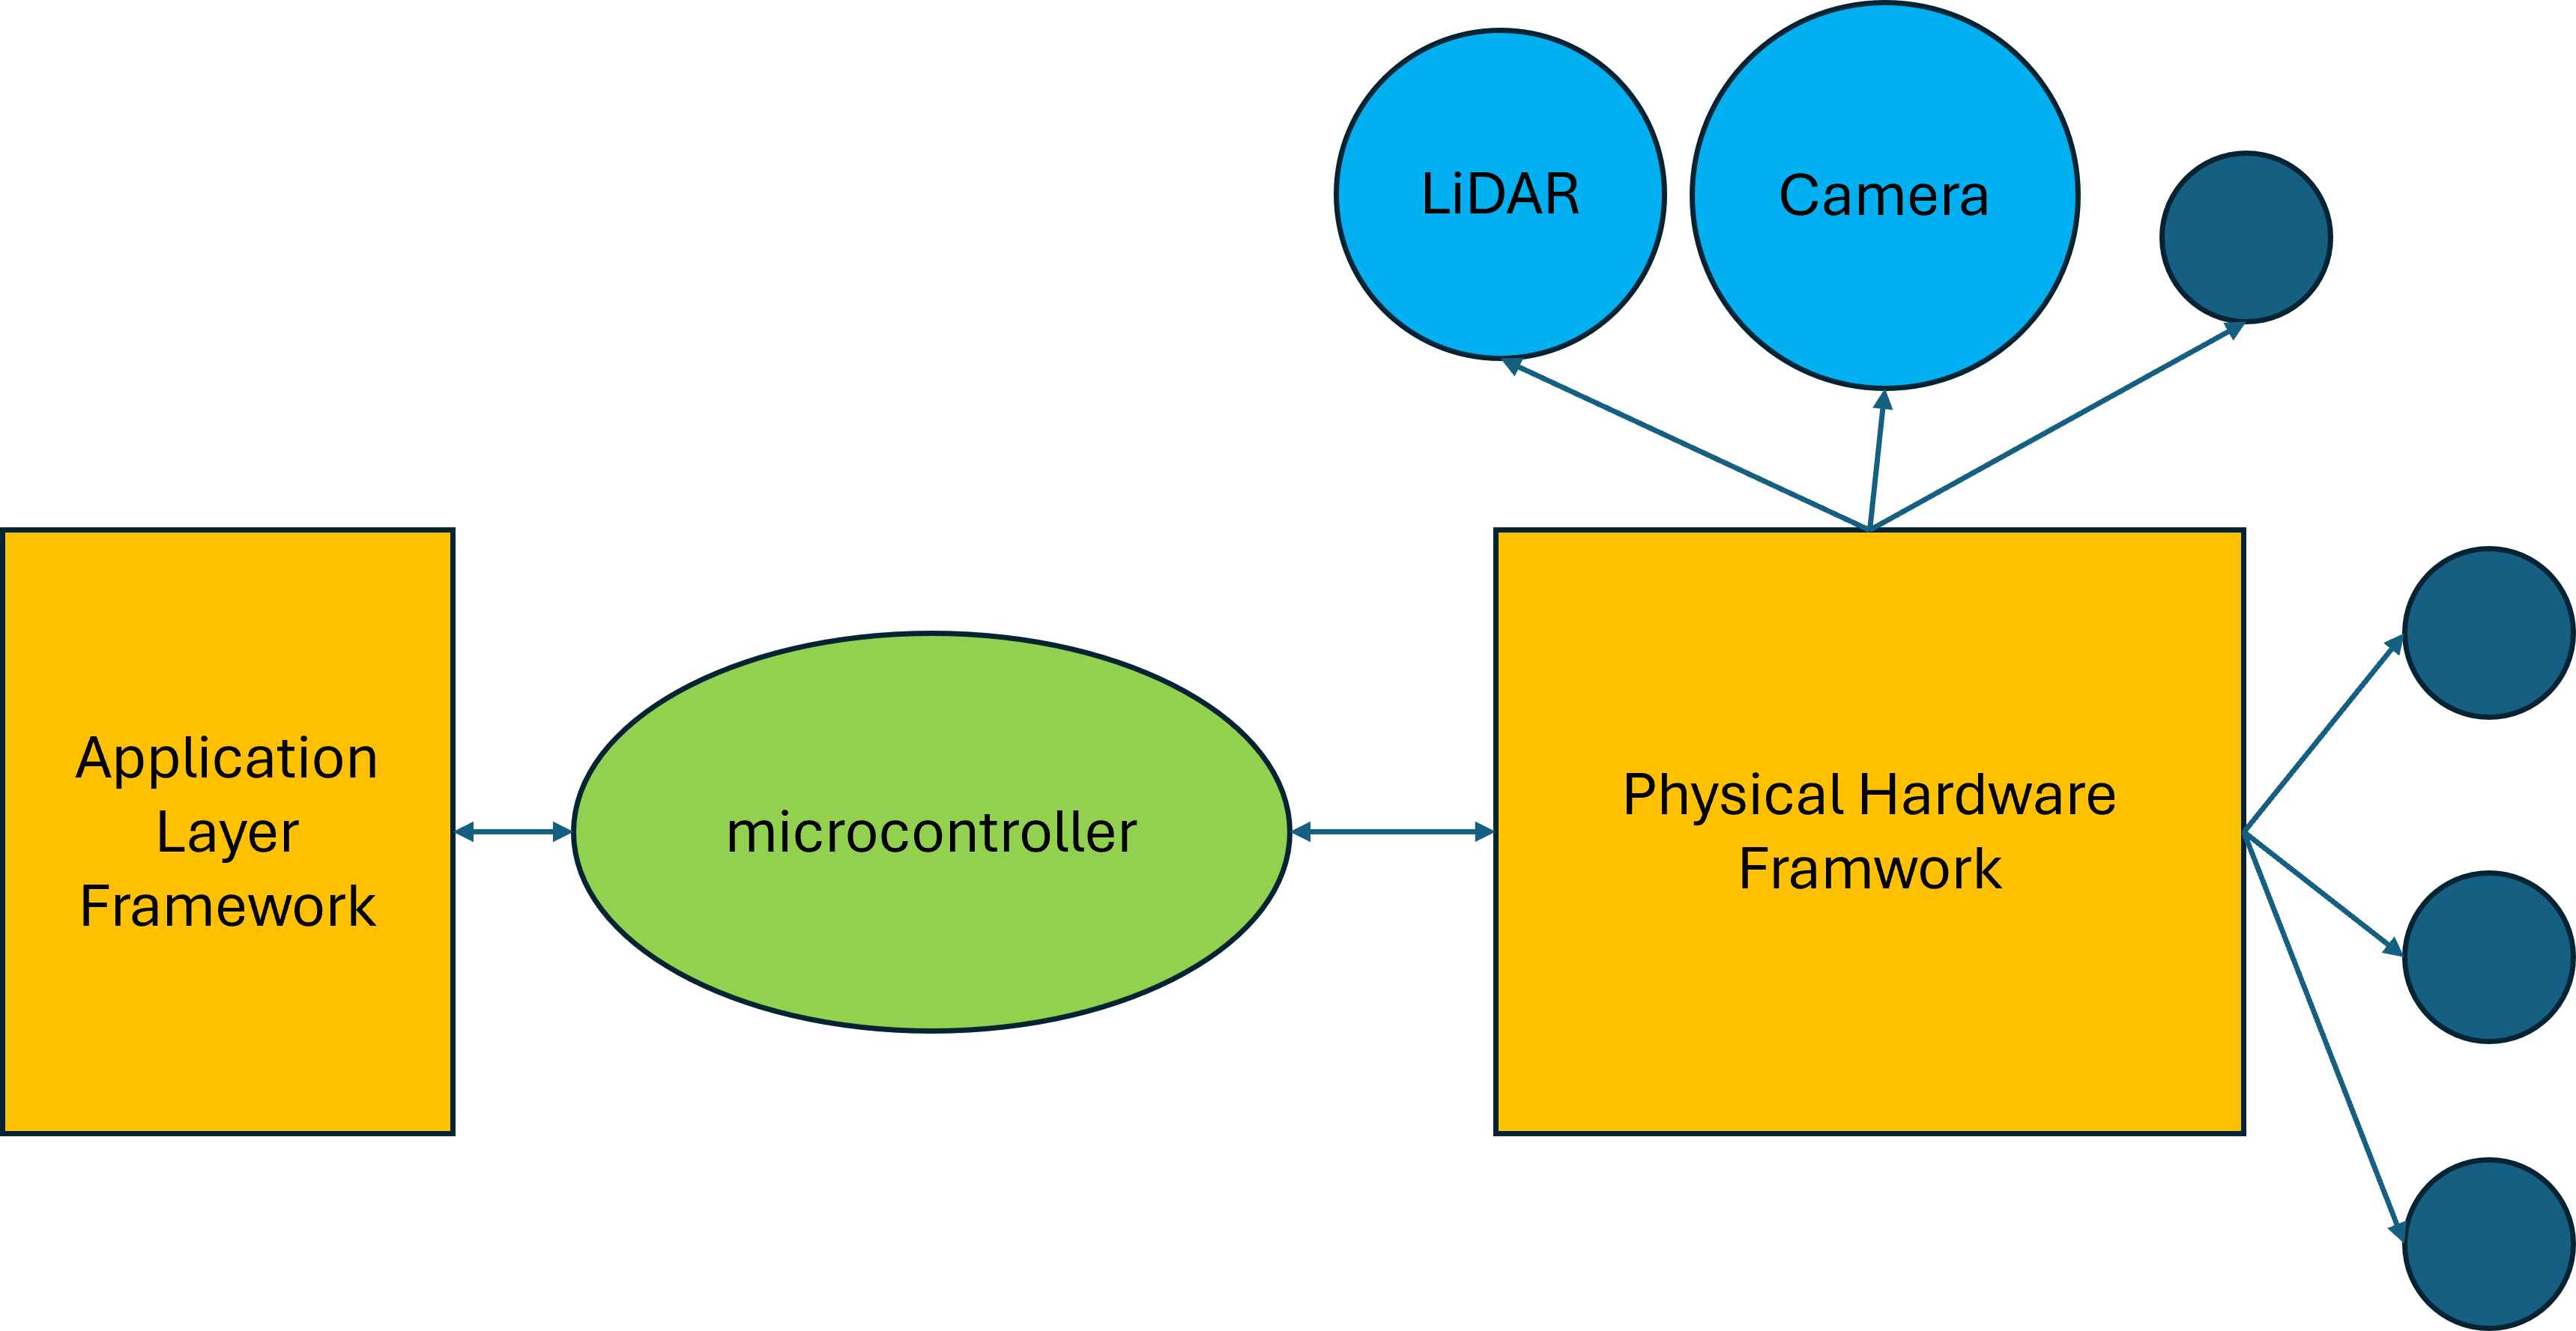
\includegraphics[width=90mm]{./pic/pic3_new_arc.png}}
\caption{the new architecture of SDL tools with the parallel frameworks. Application Layer Framework is the work of present SDL tools.}
\label{fig3}
\end{figure}
\begin{figure}[htbp]
\centerline{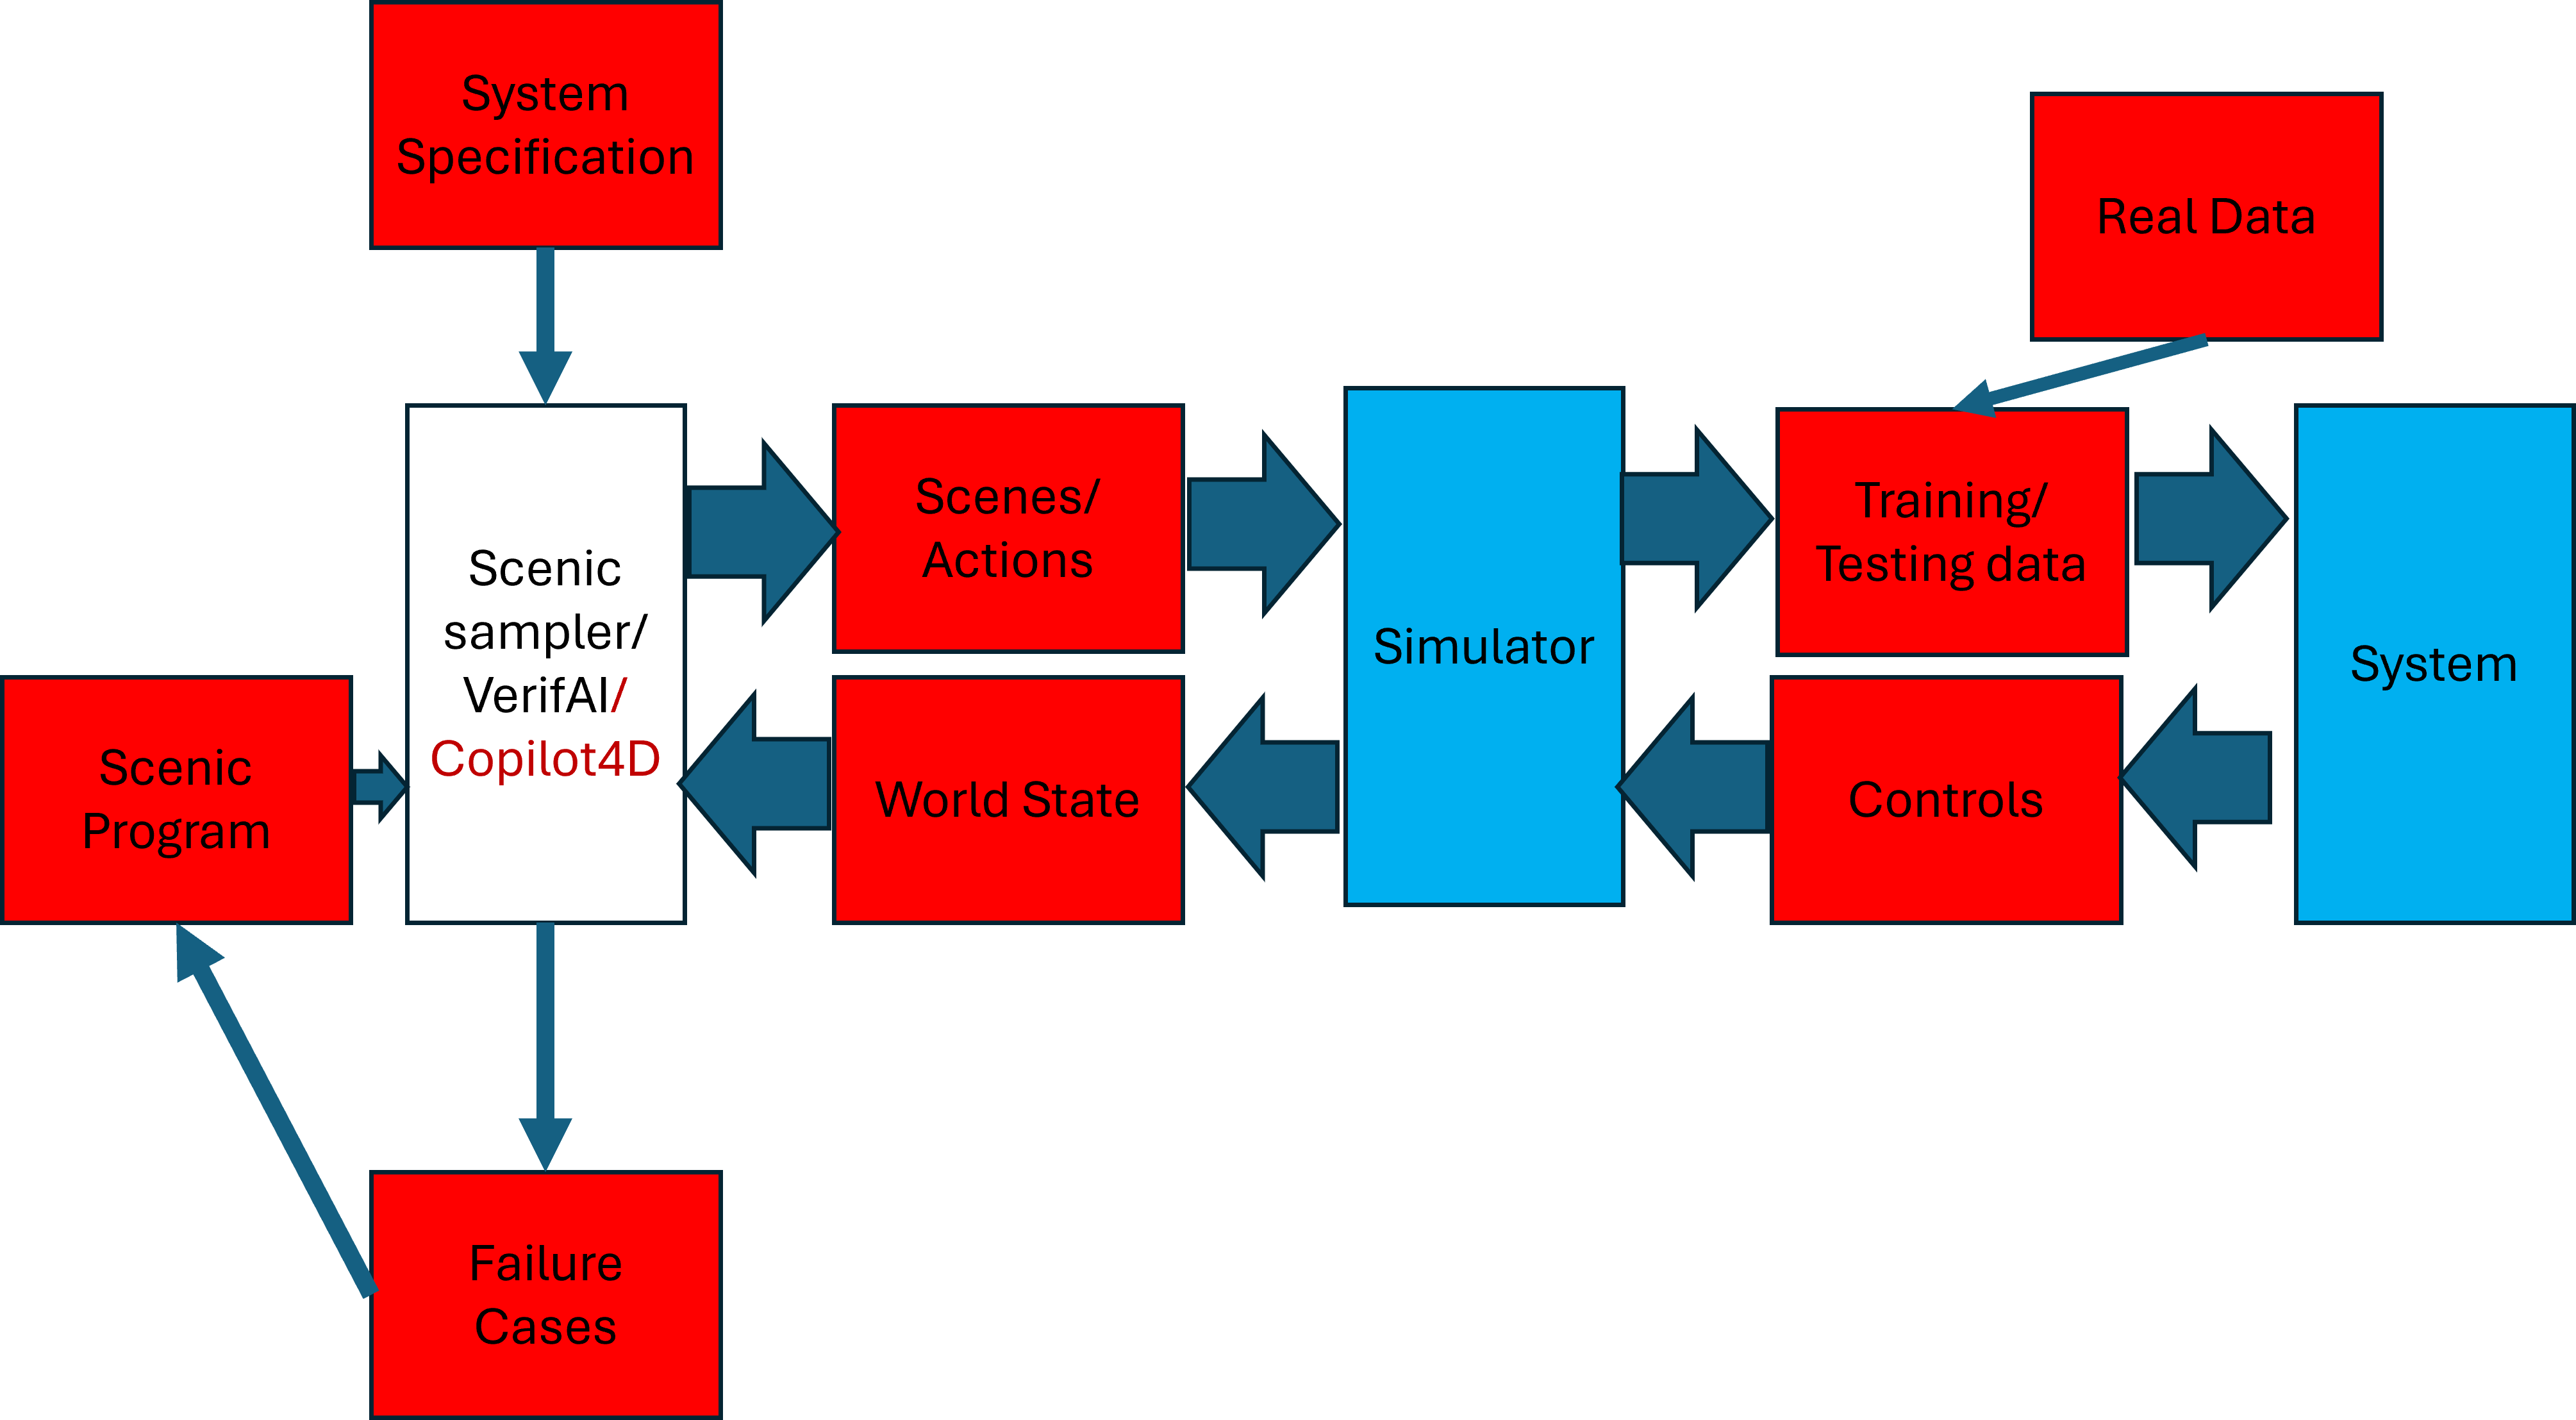
\includegraphics[width=90mm]{./pic/pic4_scenicflow.png}}
\caption{The difference part is the box with the background color white. The newly added part is models from the Physical Hardware layer, like Copilot4D.}
\label{fig4}
\end{figure}
To solve these issues, a new architecture for SDL tools can be seen in Fig.\ref{fig3}. If the work of SDL tools now is called Application Layer Framework, it is necessary to add an extra framework as physical hardware to run parallel to the framework now. Additionally, to test the success of attacks on devices, there should be an extra data processing center, like a microcontroller, between these 2 frameworks to generate the necessary actions for the vehicles. Under the physical hardware framework, there are several parallel processes, like LiDAR and cameras. Each device under this framework has 2 basic perspectives: \textbf{attack} and \textbf{protection}. Then, the flow of the SDL tools can be seen in Fig.\ref{fig4}. The difference is the added models for this new Physical Hardware framework. The whole design will refer to the microkernel system concept, so the current work of SDL tools should stay as a kernel while all the other new considerations of Physical hardware are removable components. Consequently, from the perspective of programs, if the users do not want to test the Physical Hardware Layer, it can still run as an original application. Otherwise, the microcontroller will then be invoked and generate the command, like "Avoiding Collision", into the Application Layer Framework while receiving the hazard signals from the Physical Hardware Framework. The basic commands in this new framework should then be discussed with different devices. Here, only the LiDAR proposal will be presented. For LiDAR, the way of attack is using a laser with different positions, properties of a laser, and length of period. The attackers can be limited to sitting inside another car  $\mathrm {B}$, so the positions and directions of malicious lasers always have the same property as the car $\mathrm {B}$. As for the last two properties, they are easy to simulate with flexibility of input. The way of protection can then be simultaneous laser firing, timing randomization or pulse fingering. Because the set-up for the experiments of these settings has been carried out, several pre-trained models can be acquired by conducting these experiments \cite{b2}. During the runtime, the pre-trained models based on the real experiments will then be used to verify the security issues. Similar to SCENIC, the actions can also be added in this framework, but here, only the action "Signal the Hazard to Microcontrollers" will be considered. Users can choose under which conditions this action should be performed as SCENIC has shown. All the other devices can follow a similar procedure and find out the corresponding commands and models if they exist. Therefore, a systematic way to build up a scenario based on attacks in the Physical Hardware Layer has been created by this proposal. In the end, to verify cybersecurity issues of AVs in more general ways, the attack models based on several devices should also be taken care of. Accordingly, each component within this new framework will also have the property of "dependency". During the runtime, the consistency of different devices within the same set of dependency should be retained. Distinguishing the different disjoint set could be solved by the usage of the Union-Find Data structure. For example, the dependency property of the LiDAR component will include cameras, so if there exists inconsistency between these 2 devices, then the attack is detected and the action of sending Hazard signals will be locked up. In this case, the attack considering consistency, like the Frustum Attack, could then be tested many times so that the researchers should find a solution more easily.

\section{Conclusion}
This work summarizes the challenges SDL tools face and proposes a systematic way to build up scenarios based on attacks. In the future, while more precise models have been developed and more attacks have been come up with, the concept of microkernel in this work could become quite useful in filtering out the outdated components and plug-in more advanced ones. Generally speaking, the improvements of SDL tools have still a long way to go. Such as SDL tools have not yet considered some natural dangers: if it is raining, the probability of skidding should be high. Moreover, if it is foggy, the functionality of Physical Hardware will be hindered by that. Therefore, the future of SDL tools is not only about broader considerations for layers but also deeper considerations within the current work.

\begin{thebibliography}{00}
\bibitem{b1}Hallyburton, R. Spencer, et al. "Security analysis of {Camera-LiDAR} fusion against {Black-Box} attacks on autonomous vehicles." 31st USENIX Security Symposium (USENIX Security 22). 2022.
\bibitem{b2} Sato, Takami, et al. "LiDAR Spoofing Meets the New-Gen: Capability Improvements, Broken Assumptions, and New Attack Strategies." ISOC Network and Distributed System Security Symposium (NDSS). ISOC, 2024.
\bibitem{b3}Zhang, Lunjun, et al. "Learning unsupervised world models for autonomous driving via discrete diffusion." arXiv preprint arXiv:2311.01017 (2023).
\bibitem{b4} Chen, He, et al. "Generating autonomous driving test scenarios based on OpenSCENARIO." 2022 9th International Conference on Dependable Systems and Their Applications (DSA). IEEE, 2022.
\bibitem{b5} Eykholt, Kevin, et al. "Robust physical-world attacks on deep learning visual classification." Proceedings of the IEEE conference on computer vision and pattern recognition. 2018.
\bibitem{b6} Fremont, Daniel J., et al. "Scenic: A language for scenario specification and data generation." Machine Learning 112.10 (2023): 3805-3849.
\bibitem{b7} Hataba M, Sherif A, Mahmoud M, Abdallah M, Alasmary W. Security and privacy issues in autonomous vehicles: A layer-based survey. IEEE Open Journal of the Communications Society. 2022 Apr 25;3:811-29.
\bibitem{b8} "Ultra Puck Surround View Lidar Sensor — Velodyne Lidar," https://velodynelidar.com/products/ultra-puck/.
\bibitem{b9} "XT32 - HESAI," https://www.hesaitech.com/en/XT32.
\bibitem{b10}"datasheet-rev06-v2p3-os1.pdf," https://data.ouster.io/downloads/data sheets/datasheet-rev06-v2p3-os1.pdf.
\bibitem{b11}ASAM  OpenSCENARIO:  User  Guide  [EB/OL].[2022-05-13]. https://www.asam.net/index.php?eID=dumpFile\&t=f\&f=4908
\&token=ae9d9b44ab9257e817072a653b5d5e98ee0babf8
\bibitem{b12}Elmquist A, Negrut D. Modeling cameras for autonomous vehicle and robot simulation: An overview. IEEE Sensors Journal. 2021 Oct 8;21(22):25547-60.
\bibitem{b13}Chang H, Zhang H, Jiang L, Liu C, Freeman WT. Maskgit: Masked generative image transformer. InProceedings of the IEEE/CVF Conference on Computer Vision and Pattern Recognition 2022 (pp. 11315-11325).
\end{thebibliography}

\end{document}
